\chapter{Human action classification}
\label{chap/act}

\section{Introduction}
\label{sec/act/intro}

% Done 
Recognising human activities from videos is regarded as a challenging problem in comptemporary computer vision research. 
It has attracted much attention recently due to the popularity of web-scale video databases, such as YouTube. 
The task of video-based human action recognition is regarded as a multi-class classification problem of 3D, time-varying (spatiotemporal) data. 
It has been widely studied for different applications, including human-computer interaction, digital entertainment, visual surveillance and automatic video indexing.  
Despite the popularity of video-based analysis in computer vision research, several issues still remain unresolved for realising its potentials: 

% Done 
\paragraph{Run-time performance in realistic recognition systems} Run-time efficiency is of vital importance for real-world object recognition systems. 
While real-time action classification is required by many time-critical applications, existing algorithms seldom take computational complexity into full consideration. Current state-of-the-art solutions focus on the final classification accuracy in the testing stage. They reported promising results on standard human action datasets \cite{Kim2007, Lin2009, Liu2008, Willems2009}. However, such solutions are not as efficient when they are applied to realistic applications, as they either employ sophisicated algorithms or complex features to maximise recognition accuracy at the expense of increased computation time. To summarise, there exists a trade-off between classification accuracy and run-time performance, designing a suitable algorithm for video-based human action analysis is a challenging engineering problem.  

% Done 
\paragraph{Responsive action recognition}  
For many applications such as human-computer interface and video surveillance, it is necessary to classify an action within a short response time, \ie lookahead time, in order to perfrom a promptly feedback to the actions observed. 
Their recognition algorithms are often repurposed from existing classification algorithms for 2D images. They have been adopted and proved effective in early video-based action recognition research, such as \cite{Schuldt2004, Dollar2005}.  
Traditional action recognition systems consider the testing video as a single 3D object. 
Typically, an class label is assigned after sufficient features are extracted from the entire testing video, or with a large lookahead. Tt is necessary to minimise the lookahead time required for time-critical tasks, still there are few attempts to improve the designs of existing action recognition systems.  
Schindler and van Gool \cite{Schindler2008} have shown that, by using appropriate spatiotemporal features, human actions could be recognised from very short video sequences (1--7 frames) with a promising accuracy comparable to the state-of-the-arts.

% done 
\paragraph{Spatial and temporal structures}
Human activities can be considered as a sequence of time-varying poses, spatiotemporal structure of actions is therefore a discriminative feature for action recognition.  
While structural information is a useful cue for the task, it is often overlooked by traditional action recognition approaches.  
Many existing methods are derived from the standard ``bag-of-words'' model in image recognition, \eg \cite{Schuldt2004, Dollar2005, Laptev2008, Niebles2008}, which has proved effective for action recognition owing to its rich discriminative power of local appearance information and its inherent benefits to cope with scaling, translation and cluttered backgrounds. 
It, however, neglects the spatial and temporal structure among features. 
When a testing video sequence is represented as a unordered set of visual codewords, all structural information of features is discarded. 

\subsection{Contributions}

% Done 
Addressing the aforementioned challenges, this chapter presents a novel method for real-time human action classification. The major objective of the proposed approach is to recognise human actions in monocular videos quickly in a short response time, while at the same time attaining state-of-the-art accuracies. To this end, this method intends to fully utilise both appearance and structure in short, overlapping video snippets as in \cite{Schindler2008}. The main contributions of the proposed method are threefold:  

% Done 
\paragraph{Learning visual codebooks via semantic texton forest} 
Inspired by the work of Shotton \etal \cite{Shotton2008}, the proposed system extends semantic texton forests (STF) from 2D image segmentation to human action classification. STF is a variant of randomised decision forest \cite{Ho1995, Amit1997, Breiman2001} that encodes textons to multiple visual codewords. STF is capable of learning a powerful codebook without computing expensive local descriptors, and without performing costly k-means clustering as in traditional action recognition algorithms. It operates directly on spatiotemporal video patches without computing expensive local descriptors or filter-bank responses, such as 3D-SIFT descriptors \cite{Scovanner2007}, non-negative matrix factorisation \cite{Wong2007}, histogram of gradient (HOG) \cite{Schuldt2004, Laptev2008} and histogram of optical flow (HOF) descriptors \cite{Riemenschneider2009}. 
In addition to faster training and testing time, Moosmann \etal \cite{Moosmann2007} also suggested that decision forest codebooks showed improved robustness to background clutter compared with traditional flat codebooks such as k-means algorithm, hence they can attain a better recognition accuracy.  

%Firstly, inspired by the work of Shotton \etal \cite{Shotton2008}, we extend the use of semantic texton forests from 2D image segmentation to spatiotemporal analysis. STFs are ensembles of random decision trees that translate interest points into visual codewords. In our method, STF performs directly on video pixels without computing expensive local descriptors and efficiently generates codewords. As well as being faster than a traditional flat codebook such as k-means clustering, STF achieves high effectiveness comparable to that of existing approaches.  As far as we are aware, this is the first method that uses STF in action recognition studies.

% Done 
\paragraph{Combining structural and appearance information}
This chapter presents the pyramidal spatiotemporal relationship match (HSRM), building on the work of Ryoo and Aggarwal \cite{Ryoo2009}.  
HSRM describes both local appearance and structural information of visual codewords, such that the subsequent action classifier recognises short video snippets to minimise classification delay. 
Feature histograms are compared using intersection in \cite{Ryoo2009}. 
Since plain histogram intersection is sensitive to noise and appearance error, pyramidal match kernel \cite{Grauman2005} is introduced to alleviate this problem. 
Taking advantage of the inherent hierarchical structure of semantic texton forests, instead of representing a video snippet as an unordered set of codewords, HSRM takes the spatiotemporal relationship among individual local feature points into account. 
Despite using only simple feature and classifier (video patches and decision trees), the proposed HSRM still achieves promising speed and accuracy by utilising both appearance and structures of human actions. 

% Secondly, the method combines structure and local appearance information based on STF. This results into a richer description of human actions, hence actions can be classified in very short video sequences. Building on the work of Ryoo and Aggarwal \cite{Ryoo2009}, we introduce the multi-pyramidal spatiotemporal relationship match (HSRM). In the original approach, structural information of spatiotemporal features are matched linearly. Quantization errors affect the robustness of recognition results. Taking the inherent benefit of the hierarchical structure of semantic texture forest, a pyramidal match kernel \cite{Grauman2005} is employed to alleviate the quantization problem. A fast and effective classifier, namely k-means forest classifier, is also proposed.

% Done 
\paragraph{Fast classification using k-means forest} 
The proposed framework employs k-means forest to classify snippets from testing videos. 
K-means forest is an ensemble of k-means decision trees, which was originally introduced by Muja and Lowe \cite{Muja2009} for approximate nearest neighbour classifier. In this work, it is repurposed to an efficient k-nearest neighbour classifier. Instead of the Euclidean kernel, HSRM is employed as the matching kernel for learning the k-means forest classifier.  
Subsequently, the recognition accuracy is further refined by adaptively combining the k-means forest and the traditional bag-of-semantic-texton method in \cite{Shotton2008} using an adaptive weighting scheme. 
As a result, the proposed combined classification algorithm demonstrates a high accuracy comparable to that of existing state-of-the-arts, whilst simultaneously achieving real-time performance. 

%Done 
\paragraph{VFAST spatiotemporal interest point detector} 
The 3D version of FAST interest point detector, namely Video-FAST (VFAST), is designed to detect sptaiotemporal interest points in training and testing videos \cite{Yu2013b}.   
The VFAST interest points are detected by directly comparing intensities in the video sequences.
Similar to FAST \cite{Rosten2010}, the VFAST detector can be further accelerated by learning a decision tree-based corner detector from training videos \cite{Rosten2010}. 
VFAST features are relatively faster than the traditional 3D interest points by Laptev \cite{Laptev2005} and Dollar \etal \cite{Dollar2005}, it is therefore suitable for real-time application. Performance evaluations for 3D interest points are discussed in chapter \ref{chap/eval}.  
The VFAST interests point also produce a denser feature set than spatiotemporal interest points in \cite{Laptev2005, Dollar2005}. It is suggested that a densely sampled visual codebook improve recognition performance \cite{Nowak2006}. 
Given a denser set of interest points, action labels can be classified from a shorter sequence without sacrificing too much recognition accuracy, minimising the number of lookahead frames required. 
In addition, scale-space analysis can be applied on VFAST in order to detect interest points across different scales.

% Lastly, several techniques are employed to improve the recognition speed and accuracy. A novel spatiotemporal interest point detector, called VFAST, is designed based on the FAST 2D corners{Rosten2006}. The recognition accuracy is improved by adaptively combining HSRM and the bag of semantic texton (BOST) method \cite{Shotton2008}.

% The rest of the chapter is structured as follows: In section \ref{sec/act/relatedwork}, related work are reviewed and, in section \ref{sec/act/overview}--\ref{sec/act/combine}, the proposed methods are detailed. Evaluation results are reported and discussed in Section \ref{sec/act/experiments} and the conclusion is drawn in Section \ref{sec/act/discussion}.

\section{Related work}
\label{sec/act/relatedwork}
% Done 

Machine recognition of human activities has been a long-lasting topic in computer vision research since the seventies, \eg moving light display \cite{Johansson1973}. Early approaches to human activity analysis were reviewed by C\'edras and Shah \cite{Cedras1995}, Moeslund and Granum \cite{Moeslund2001} and Turaga \etal \cite{Turaga2008}. Contemporary action recognition algorithms are reviewed by Poppe \cite{Poppe2010} and Weinland \etal \cite{Weinland2011}.   

State-of-the-art action recognition methods have shown the effectiveness of local appearance-based features, as the bag-of-words model is particularly popular in the literature \cite{Dollar2005, Riemenschneider2009, Niebles2008, Schuldt2004, Wong2007}.
In a typical ``bag-of-words'' object recognition model, input feature vectors are quantised into visual codewords by a learned codebook. Each object is represented by its frequency list, \ie histogram of visual codewords. A classifier is then trained to assign labels to the testing objects.

% Done 
For action classification, a large codebook, \eg up to thousands of codewords, is favourable to ensure a good recognition accuracy. However, computational load and memory requirement also increase with codebook size. With respect to learning algorithms, feature quantization methods by a large flat codebook, such as k-means, is computationally heavy. Furthermore, an oversized codebook is vulnerable to high quantisation errors and overfitting. As a result, alternative approaches to codebook learning have been investigated to increase the efficiency and robustness for action classification. 
Moosmann \etal \cite{Moosmann2007} suggested learning a fast visual codebook as a randomised clustering forest. Since then tree-based codebook has been increasingly adopted in various object recognition tasks, including scene recognition \cite{Bosch2007} and semantic segmentation \cite{Shotton2008}, owing to its superior efficiency and generalisation power.
There exist two main advantages of using a tree-based codebook for object recognition. 
Firstly, decision trees can be highly parallelised for efficient computation, which is essential for time-critical applications. Secondly, given a feature vector, a decision tree produces multiple visual codewords at different levels, increasing the robustness of visual codeword matching. 

% Done 
As a variant of tree-based codebook, Oshin \etal \cite{Oshin2009} recognised human actions by describing the spatial distribution of interest points by random ferns.  
Lin \etal \cite{Lin2009} used a prototype tree to encode holistic motion-shapes descriptors. 
Mikolajczyk and Uemura \cite{Mikolajczyk2008} accelerated codebook testing time by learning clustering trees from the results of k-means clustering. 
Hierarchical codebooks enable fast vector quantisation during testing, however, the expensive features and classifiers used in \cite{Lin2009, Mikolajczyk2008} make the overall processes still heavy.

% Done 
Codeword histograms are orderless in the bag-of-words model. 
Typical bag-of-words algorithms contain only encoded appearance information of local features.  
% Standard bag of words models contain only local appearance information. 
Whilst structural context is useful in describing some action classes, it is often omitted in current action recognition methods.
On the other hand, some studies have implied that structural or holistic features can be as effective as local features. 
For instance, Gorelick \etal \cite{Gorelick2007} considered human actions as 3D space-time shapes, which are built from foreground silhouettes in the testing videos. Fathi and Mori \cite{Fathi2008} recognised actions using global mid-level features built from optical flow in segmented 3D patches. Kim \etal \cite{Kim2007} applied canonical correlation analysis to describe human actions in videos. The major limitation of these approaches is that segmentation or action detection is required before the extraction of holistic features.  

% Done  
Some recent studies attempted to augment action recognition algorithms by considering structural information in addition to local appearances. 
Savarese \etal \cite{Savarese2008} proposed correlograms to describe the co-occurrences of visual codeword in a space-time neighbourhood. Spatial correlograms were also used in the work by Liu and Shah \cite{Liu2008} to encode structural information of visual word clusters.  
Wong \etal \cite{Wong2007} presented the pLSA-ISM model, which is an extension of the pLSA topic model \cite{Fergus2005} with additional spatial information from implicit shape model (ISM). 
Tran \etal \cite{Tran2008} extracted silhouettes and motion templates and classified action using metric learning.  
Zhang \etal \cite{Zhang2008} designed motion context, which is a spatiotemporal hollistic feature based on the shape-context descriptor.  

% Done  
Nevertheless, the structural relationship among local features are not effectively described in the above techniques. 
Some approaches \cite{Wong2007,Tran2008, Zhang2008} encode local features with respect to a canonical reference frame, \eg a rectangular region-of-interest. In order to detect actions, they require segmentation or additional pre-processesing, which are often computationally expensive.
Addressing this issue, Ryoo and Aggarwal \cite{Ryoo2009} proposed the spatiotemporal relationship match (SRM) that encodes spatiotemporal relationship between visual codewords using a set of pairwise rules. Kovashka and Grauman \cite{Kovashka2010} exploited structural information by learning an optimal neighbourhood measure of interest points. 
Albeit high recognition accuracy, speed and quantisation errors remain the main issues for these approaches because flat k-means codebooks are used.   

% Done 
New machine learning techniques have been introduced to improve the accuracy of different action classification tasks.  
For instance, pyramid match kernel (PMK) \cite{Grauman2005} has recently been used in object detection and image-based retrieval. PMK constructs multi-resolution, hierarchical histograms where codewords are assigned to bins according to their spatial locations. Similar points that do not match in fine resolutions have the chance to match in lower resolutions, reducing quantisation errors and enhances robustness in spatial domain. PMK has recently been applied in action classification, Liu and Shah \cite{Liu2008} matched interest points in multiple resolutions using PMK and reported improved results over flat histogram intersection kernel. 
However, PMK only performs hierarchical matching in spatial domain, the semantical similarities among codewords are not modelled.  

% Done  
As discussed in chapter \ref{chap/eval}, feature detection and representation also play an crucial role in the performances of action classification systems. Several interest points are specifically designed for spatial temporal data. For example, Laptev \cite{Laptev2005} proposed spatiotemporal interest point (STIP), which is extended from 2D Harris corner detection algorithm. Dollar \etal \cite{Dollar2005} then enhanced the density of STIP by applying Gaussian filter in space and Gabor filter in time.  
Wong and Cipolla \cite{Wong2007a} extracted discriminative regions using non-negative matrix factorisation, decomposing videos into linear combinations of shared space-time components.
Based on salient region detection algorithm \cite{Mikolajczyk2004}, Oikonomopoulos \etal \cite{Oikonomopoulos2005} computed spatiotemporal saliency by measuring the entropy within a spherical neighbourhood. Messing \etal \cite{Messing2009} used trajectories of tracked keypoints to recognise actions from videos. 
With respect to feature descriptors, HOG and HOF are popular techniques in earlier action classification methods \cite{Dollar2005, Niebles2008, Schuldt2004}. Scovanner \etal \cite{Scovanner2007} proposed a 3D version of Lowe's popular SIFT descriptor \cite{Lowe2004}. Willems \etal \cite{Willems2009} presented an extended SURF descriptor in videos for action recognition.  
% Extra feature descriptor? 
To summarise, feature extraction is often one of the most computationally expensive processes in action classification systems. Efficient features, or descriptor-less approaches, are investigated to improve the run-time speed of action classification.  

% done 
In addition to classification accuracy, run-time performance is another essential quality for realistic huamn action recognition systems. Various techniques are developed to speed up feature extraction and classification. 
Instead of HOG and HOF, Yeffet and Wolf \cite{Yeffet2009} computed dense local trinary patterns, which is an efficient feature derived from local binary patterns for texture analysis and face recognition \cite{Ahonen2006}. 
Gilbert \etal \cite{Gilbert2009} proposed a fast multi-action recognition algorithm by finding patterns of dense 2D Harris corners with a data-mining algorithm.
Patron-Perez and Reid \cite{Patron2007} designed a probabilistic classifier that recognised actions continuously with a sliding window. 
Bregonzio \etal \cite{Bregonzio2009} considered actions as clouds of points, efficient classification was done by analysing histogram of point clusters. 
Regarding the classification step in existing systems, standard classifiers are often used.
K-nearest neighbour classifier, support vector machines and boosting were among the most widely adopted algorithms. New models were proposed to accelerate the classification process, such as k-NN approximation using decision trees \cite{Lin2009}, randomised ferns \cite{Oshin2009} and Markov chains \cite{Messing2009}.   
Although real-time performances have been reported by these methods, their computation bottlenecks in feature extraction and vector quantisation have not been addressed. 

\section{Overview of the proposed method} 
\label{sec/act/overview}

%done 
An overview of the proposed action classification system is illustrated in figure \ref{fig/act/flow}. 
Salient points in videos are first detected by the proposed VFAST detector. 
Spatiotemporal patches, extracted from the detected interest points, are quantised into visual codewords using a trained semantic texton forest, which is explained in section \ref{sec/act/stf}. 
%Using pairwise codewords and their spatiotemporal associations, histograms that capture both local-appearance and structural information are constructed.
Visual codewords are paired according to a predefined set of association rules, capturing both local appearance and structural information of training and testing videos.  
Preliminary recognition is performed efficiently using a k-means forest classifier with HSRM \ref{sec/act/HSRM}. 
The results from k-means forest are adaptively combined with the prior-art that uses the bag of semantic texton (BOST) and random forest classifier.
The feature extraction phase of the proposed framework is flexible. 
Depending on the target application, simple spatiotemporal video patches can be replaced by more discriminative local features, such as HOG or tracked trajectories.

\begin{figure}[ht]
	\centering  	
	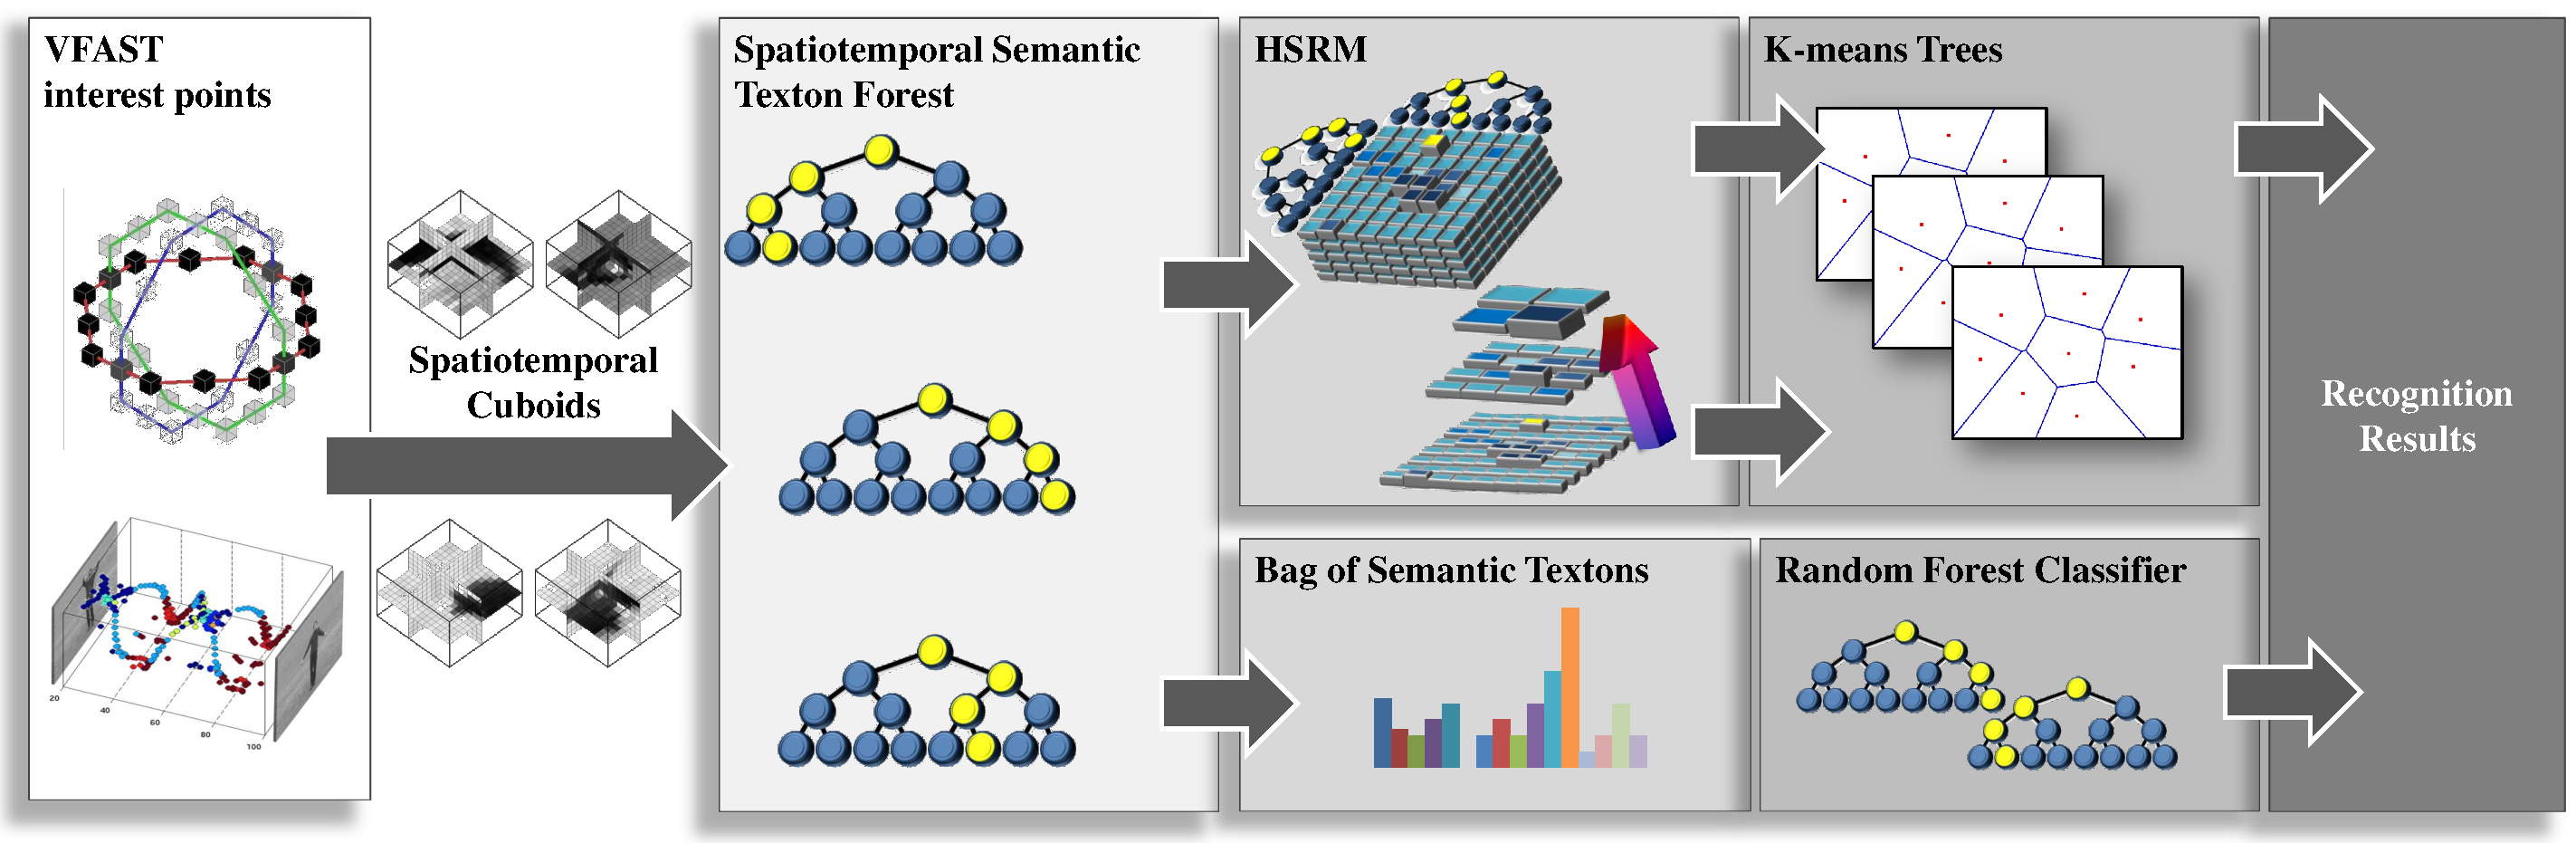
\includegraphics[width=1.0\linewidth]{fig/act/fig1_new4.pdf}
	\caption{Overview of the proposed approach}
	\label{fig/act/flow}
\end{figure}

\section{VFAST interest point detector}
\label{sec/act/fastest}
% DONE 
Video FAST (VFAST) interest points are obtained by extending the FAST corners \cite{Rosten2006} into a spatiotemporal domain. It considers pixels in three orthogonal Bresenham circles $C$ with radii $r_{XY}$, $r_{YT}$ and $r_{XT}$ on $XY$, $YT$ and $XT$ planes respectively.
For a spatiotemporal volume $\vpatch$, FAST saliency is detected on a plane if there exist $n$ contiguous pixels on the circle which are all brighter than the intensity of the reference voxel $\vpatch(x,y,t)$ plus a predefined threshold $\delta^{FAST} \in \{ t_{XY}, t_{XT}, t_{YT} \}$, or all darker than $\vpatch(x,y,t)$ minus $\delta^{FAST}$. An interest point is detected when the reference pixel shows both spatial ($XY$ plane) and temporal ($XT$ plane or $YT$-plane) saliency. The steps of computing VFAST interest points are described in algorithm \ref{algo/act/vfast}.

%DONE 
\begin{algorithm}
\caption{VFAST spatiotemporal interest point detector}
\label{algo/act/vfast}
\begin{algorithmic}
	\REQUIRE $[x,y,t] = $ voxel coordinates
	\REQUIRE $r_{XY},r_{XT},r_{YT} = $ Radii of Bresenham circles
	\REQUIRE $n = $ Contiguous threshold
	\REQUIRE $\delta^{FAST} = $ Intensity threshold
	\STATE $C_{XY}(r_{XY}),C_{XT}(r_{XT}),C_{YT}(r_{YT})$ = Pixels of Bresenham circles
	\STATE $FAST_{XY} = ( C > \vpatch(x,y,t)+t_{XY}\quad or\quad C < \vpatch(x,y,t)-\delta^{FAST}_{XY} )$
	\STATE $FAST_{XT} = ( C > \vpatch(x,y,t)+t_{XT}\quad or\quad C < \vpatch(x,y,t)-\delta^{FAST}_{XT} )$
	\STATE $FAST_{YT} = ( C > \vpatch(x,y,t)+t_{YT}\quad or\quad C < \vpatch(x,y,t)-\delta^{FAST}_{YT} )$
	\IF {Number of contiguous pixels in $Saliency_{XY} \ge n$}
	\IF{(${ContiguousPixel}(FAST_{XY}) \ge n$)}
		\RETURN \texttt{TRUE}
	\ELSIF{($ContiguousPixel(FAST_{XY}) \ge n$)}
		\RETURN \texttt{TRUE}
	\ELSE
		\RETURN \texttt{FALSE}
	\ENDIF
\ENDIF
\end{algorithmic}
\end{algorithm}

% DONE
Figure \ref{fig/act/fastest} illustrates how interest points are detected using the 42-pixel V-FAST interest point detector with $r_{xy},r_{xt},r_{yt} = 3$. 

\begin{figure}[ht]
	\centering
	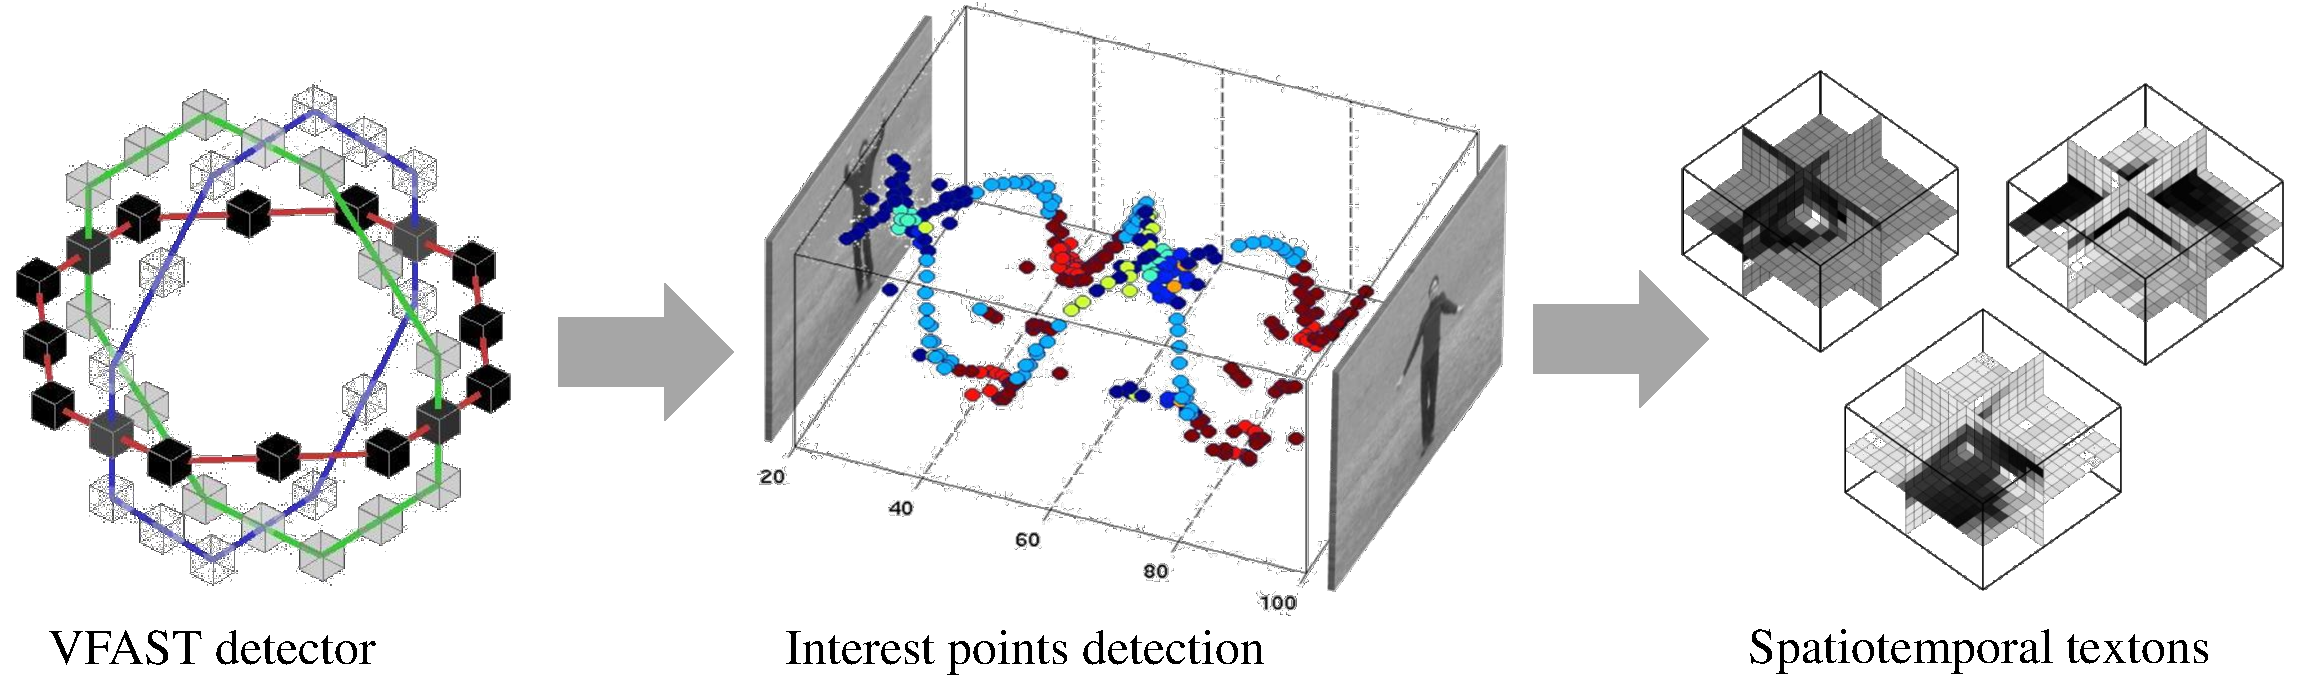
\includegraphics[width=1\linewidth]{fig/act/fig2_new.pdf}
	\caption{Detecting VFAST spatiotemporal interest points in videos}
	\label{fig/act/fastest}
\end{figure}

%\section{Random Forest}
%blah blah blah 

\section{Spatiotemporal semantic texton forest}
\label{sec/act/stf}

%done
Semantic texton forest (STF) is an ensemble of randomised decision trees which textonises input video patches into semantic textons. Instead of using as a classifier, Moosmann \etal \cite{Moosmann2007} extended random forest to vector quantisation by learning multiple tree-based codebooks. Shotton \etal \cite{Shotton2008} applied this technique in image segmentation by quantising texture patches using a STF. In this chapter, STF is used to convert video patches into visual codewords.  
It is an extremely efficient codebook, where feature vectors traverse each of the trees by simple voxel pair tests, without computing filter responses or feature descriptor. STF codebook also demonstrates higher robustness and discriminative power than k-means algorithm because it produces multiple codewords from a feature vector. 

% Done 
The training algorithm of STF is similar to that of supervised classification forest \cite{Breiman2001}. At each new node, a pool of candidate split functions are generated randomly, a split function is selected from the pool, by maximising the information gain $\mathrm{IG}(\cdot)$ in the current training data. 
\begin{equation}
	\begin{aligned}
		\histogram(\tdata) & = -\sum_{c \in C} \frac{|\tdata[c]|}{|\tdata|}\log_{2}(\frac{|\tdata[c]|}{|\tdata|})\\ 
		\mathrm{IG}(\tdata) & = \histogram(\tdata) - \frac{|\tdata_{l}|}{|\tdata|}\histogram(\tdata_{l}) - \frac{|\tdata_{r}|}{|\tdata|}\histogram(\tdata_{r})
	\end{aligned}
	\label{eqn/act/ig}
\end{equation}
where $\histogram(\tdata)$ is the information entropy of the current dataset $\tdata$, $\tdata[c]$ denotes the subset of $\tdata$ that belongs to class $c$. $\tdata_{l}$ and $\tdata_{r}$ are the left and right subset of $\tdata$ that are divided by the candidate split function. 
Split functions are assigned to a new node by maximising equation \ref{eqn/act/ig}. As a result, training video cuboids are clustered recursively down the decision tree. Training is stopped when the new tree nodes reach a certain depth. Algorithm \ref{c3/algo/grow} describes the recursive procedure of learning a randomised decision tree in a STF.

\begin{algorithm}
\caption{Semantic Texton Tree Node Training}
\label{c3/algo/grow}
\algsetup{indent=2em}
\begin{algorithmic}
	\STATE \hspace{-2em} \textbf{function split}($\tdata$, $N$):
	\STATE Generate a pool of candidate split functions in $\Theta = \{ \theta_{1},\dots,\theta_{|\Theta|}\}$
	\FOR {$i = 1$ to $|\Theta|$}
	\STATE Split training data $\tdata$ using $\theta_i$;
	\STATE $\tdata_l \Leftarrow$ data points in $\tdata$ which $\theta_i$ return $0$
	\STATE $\tdata_r \Leftarrow$ data points in $\tdata$ which $\theta_i$ return $1$
	\STATE $\mathrm{IG}(\tdata) = \Delta\histogram(\tdata)$ 
	\ENDFOR
	\STATE Find the $j$-th candidate split that maximises $\mathcal{IG}(\tdata)$
	\STATE Assign $\theta_j$ to the current node 
	\IF {(Node has not reached maximum depth)}
		\STATE Create left node $N_l$
		\STATE Create right node $N_r$
		\STATE \textbf{split}($\tdata_l$,$N_l$);
		\STATE \textbf{split}($\tdata_r$,$N_r$);
	\ENDIF
	\STATE \hspace{-2em} \textbf{end function}
\end{algorithmic}
\begin{algorithmic}
	\STATE \hspace{-2em} \textbf{function grow}():
	\STATE $\tdata' = $ current training data
	\STATE Add root node $N_{0}$ to tree
	\STATE \textbf{split}($\tdata'$, $N_{0}$)
	\STATE \hspace{-2em} \textbf{end function}
\end{algorithmic}
\end{algorithm}

%Done 
In the proposed action classification system, a split function $\theta(\cdot)$ is defined as the weighted difference between two voxel values in an input video patch $\vpatch$ in equation \ref{eqn/act/stftest}. 
\begin{equation}
	\theta(p) = 
	\left\{
		\begin{aligned}
			1 & \mbox{ when } w_1 \vpatch(x_1,y_2,t_1) - w_2 \vpatch(x_2,y_2,t_2) > threshold \\  
			0 & \mbox{ otherwise } 
		\end{aligned}
	\right.
	\label{eqn/act/stftest}
\end{equation}
where $\vpatch(x_1, y_1, t_1)$ and $\vpatch(x_2, y_2, t_2)$ are two randomly selected voxels from the input video patch, and $w_1$ and $w_2$ are random weightings for $\vpatch(x_1,y_1,t_1)$ and $\vpatch(x_2,y_2,t_2)$ respectively. 
% Done 
During test time, a STF acts on small spatiotemporal cuboid patches, which are extracted around the detected VFAST interest points. These video cuboids are then flattened to feature vectors, which pass down all $M$ trees in the STF. 
The forest recursively clusters these video cuboids according to the chosen split functions.  
% until reaching a certain depth in the randomised decision tree. 
The STF codebook has a size of $\codebooksize=\sum_m^M \codebooksize_m$ where $\codebooksize_m$ denotes the number of leaf nodes, \ie codewords in $m$-th tree. 
Consequently, in each decision tree, the set of video cuboids are roughly clustered into $\codebooksize_m$ groups based on their appearance, the average of cuboids within a node is called a semantic texton \cite{Shotton2008}. 
Figure \ref{fig/act/stf} demonstrates how input spatiotemporal patches are clustered into two codewords through a tree node. 

Table \ref{tab/act/codebook} summarises a quantitative comparison between STF and k-means algorithms. Relative speed is measured by computing $1$ million feature vectors with $405$ dimensions. Size of codebook $K$ is $1905$. The branching factor $b$ for k-means algorithm is $16$.

\begin{figure}[ht]
	\centering 
	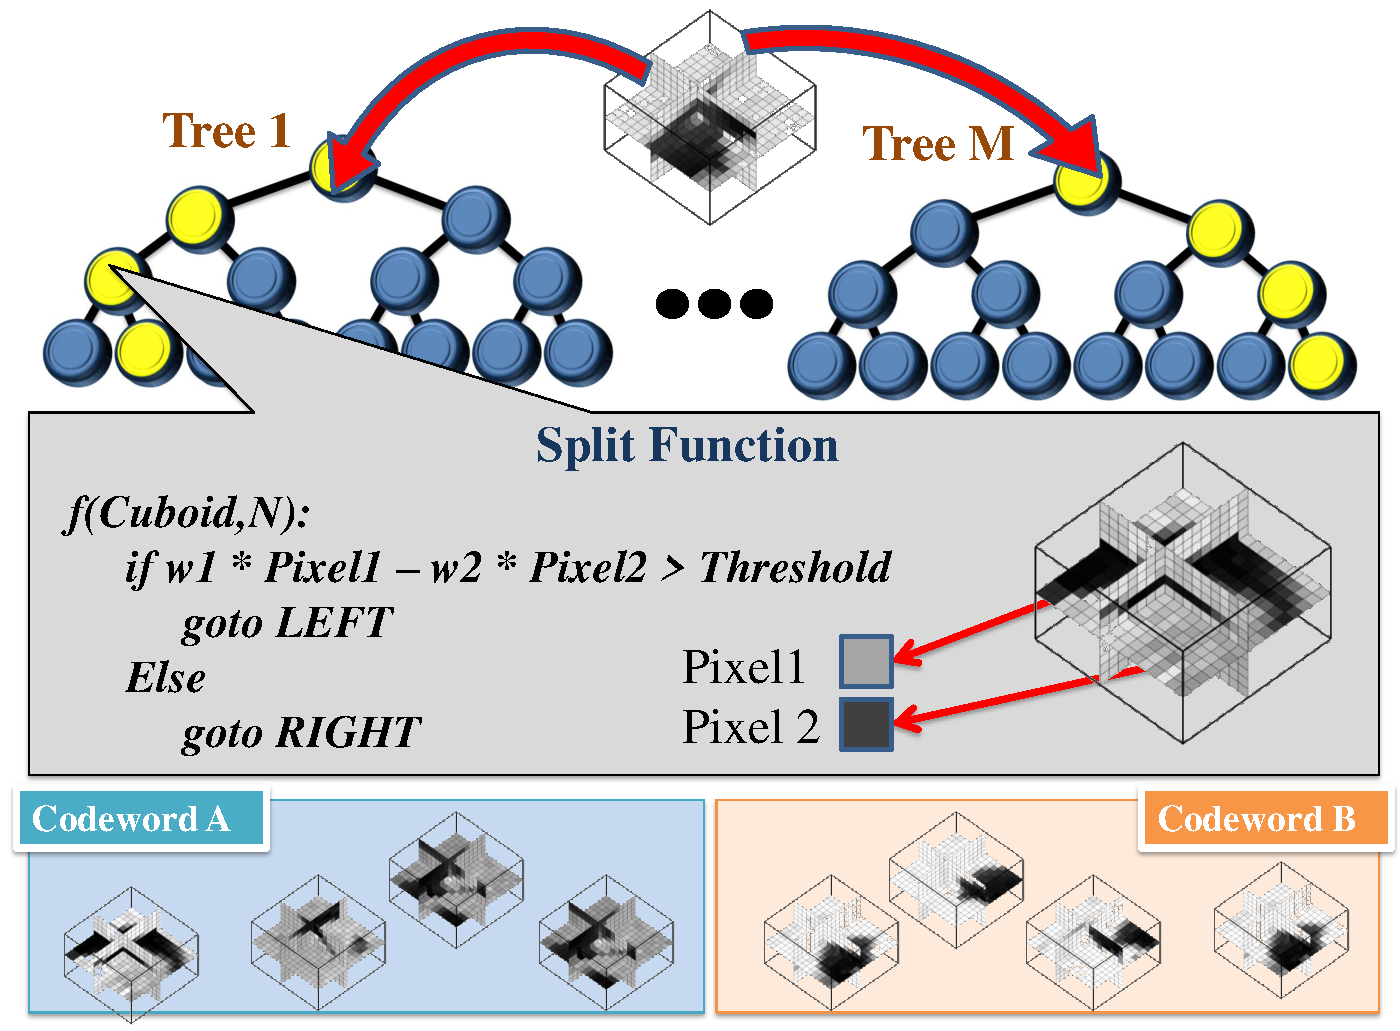
\includegraphics[width=0.8\linewidth]{fig/act/stf_new.pdf} 
	\caption{Visual codeword generation by Spatiotemporal Semantic Texton Forest}
	\label{fig/act/stf}
\end{figure}

\begin{table}
	\begin{center}
		\begin{tabular}{|c|c|c|c|}
			\hline
			\textbf{ Algorithm} & \textbf{ Copmlexity} & \textbf{ Relative Speed}* & \textbf{ Hierarchical} \\
			\hline
			k-means & $O(K)$ & $1$ & no \\
			Hierarchical k-means & $O(b\log_{b}(K))$ & $43.51$ & yes \\
			{\color{blue}{STF}} & {\color{blue}{ $ O(\log_{2}(K)) $ }} & {\color{blue}{$559.86$}} & {\color{blue}{yes}}\\
			\hline
		\end{tabular}
	\end{center}
	\caption{Quantitative comparison of semantic texton forest and k-means codebooks.}
	\label{tab/act/codebook}
\end{table}

\section{Hierarchical spatiotemporal relationship match}
\label{sec/act/HSRM}

% Done 
Hierarchical spatiotemporal relationship match (HSRM) is designed to describe both local-appearance and structural information efficiently in one histogram. 
Firstly, STF quantises local spatiotemporal volumes into visual codewords. 
Seconly, for each tree in the STF codebook, a three-dimensional histogram is constructed by analysing pairs of codewords for their spatiotemporal co-occurences, as shown in figure \ref{fig/act/hsrm} (left and middle). 
For each histogram, a novel pyramid match kernel is proposed for robust matching in figure \ref{fig/act/hsrm} (right). 
Finally, multiple pyramidal matches are then combined to classify a query video. 

Whereas the spatiotemporal relationship match (SRM) by Ryoo \etal \cite{Ryoo2009} relies on a flat k-means codebook, HSRM leverages the hierarchical properties of multiple tree-based codebooks and performs robust matching using pyramid match kernels. The tree structure offers a time-efficient way to perform semantic codeword matching between pairs of histograms \cite{Grauman2005}.

% done 
\begin{figure}[ht]
	\centering	
	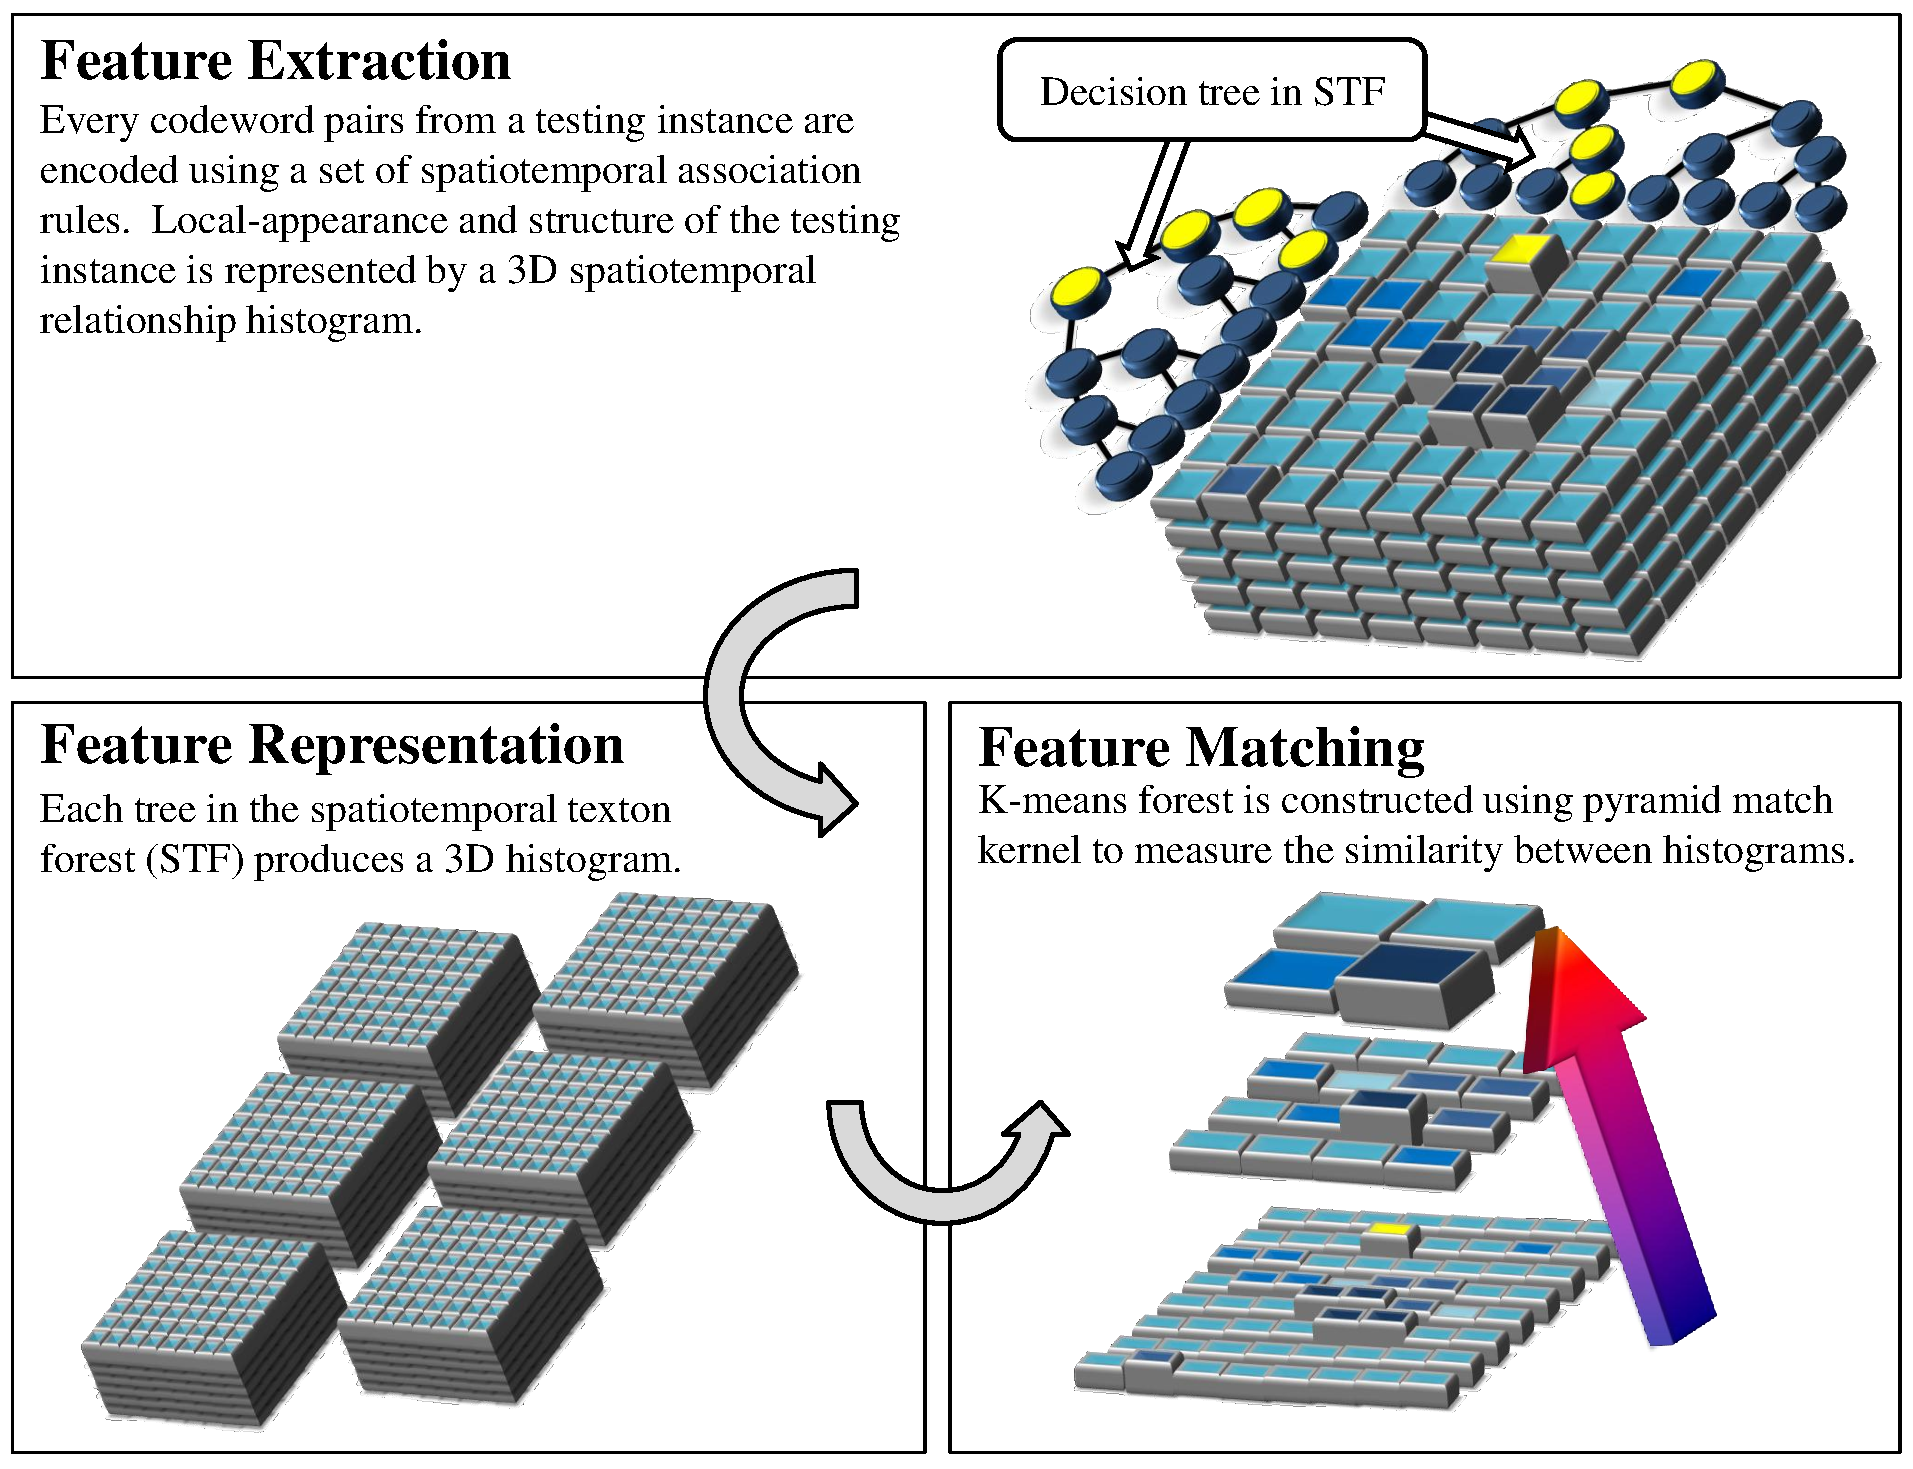
\includegraphics[width=0.9\linewidth]{fig/act/fig4_new.pdf} 
	\caption{Multi-pyramidal spatiotemporal relationship match (HSRM)}
	\label{fig/act/hsrm}
\end{figure}

\subsection{Building spatiotemporal relationship histograms}

% done 
Short video snippets are the basic input units of the proposed system, which are densely sampled from an input video.  
A set of VFAST interest points $\vfastset = \{\onevfast_{i}\}$ are localised from the snippets. Visual codewords are assigned to the interest points by the STF.   
The $i$-th encoded interest point is described as 
\begin{equation}
	\onevfast_{i} = \{x_i, y_i, t_i, l_{m,i}\}_{m=1,\dots,M}
\end{equation}
where $x_i, y_i, z_i$ represents a $XYT$-location of the feature and $\vcode_{m,i}$ is the visual codeword, \ie leaf node assigned to $\onevfast_{i}$ by the $m$-th tree. 
In the proposed system, a set of pair-wise spatiotemporal associations are designed to capture the structural relations among interest points. By analysing all possible pairs $\onevfast_i$ and $\onevfast_j$ in $\vfastset$, space-time structures of codewords are described by the following seven association rules $\mathcal{R} = \{ R_1,\dots,R_7\}$:

% done 
\begin{equation}
	\centering 
	\begin{array}{lr}
		R_{1}~{\color{blue}overlap}: & |t_i - t_j| < \mathrm{T_{o}} \\
		R_{2}~{\color{blue}before}: & \mathrm{T_{o}} < t_j - t_i < \mathrm{T_{b}} \\
		R_{3}~{\color{blue}after}: & \mathrm{T_{o}} < t_i - t_j < \mathrm{T_{a}} \\
		R_{4}~{\color{blue}nearXY}: & (|x_i - x_j| < \mathrm{T_{n}}) \wedge (|y_i - y_j| < \mathrm{T_{n}}) \\
		R_{5}~{\color{blue}nearX}: & (|x_i - x_j| < \mathrm{T_{n}}) \wedge \sim(R_{4}) \\
		R_{6}~{\color{blue}nearY}: & (|y_i - y_j| < \mathrm{T_{n}}) \wedge \sim(R_{4}) \\
		R_{7}~{\color{blue}far}: & (|x_i - x_j| < \mathrm{T_{f}}) \wedge (|y_i - y_j| < \mathrm{T_{f}}) \wedge \sim(R_{4} \vee R_{5} \vee R_{6})
	\end{array}
\end{equation}

% done 
Figure \ref{fig/act/hsrm} illustrates the construction and matching of the spatiotemporal relationship histograms using the proposed HSRM. 
A set of 3D histograms $\{ \histogram_1(\vfastset),\dots,\histogram_{M}(\vfastset)\}$ are constructed by encoding all possible pairs of feature points in $\vfastset$. The bin $\mathrm{h}_{m}(i,j,k)$ for the $m$-th tree $\histogram_{m}(\vfastset)$ corresponds to the number of matching $(\vcode_{m,i},\vcode_{m,j})$ codeword pairs by an association $R_k$. The total number of bins of $\histogram_m(\vfastset)$, \ie histogram size, is $\codebooksize_m \times \codebooksize_m \times |\mathcal{R}|$. Since the spatiotemporal histograms are sparse, their operations can be greatly accelerated using sparse matrices data structures.  

\subsection{Pyramid match kernel for HSRM}
% done 
Quantisation is a major issue of bag-of-words models for 3D object recognition tasks in general. It is often difficult to determine an optimal codebook size, which is dependent on both training and testing data. 
If a codebook is too small, useful information is discarded due to quantisation error, affecting its discriminative power. 
Oppositely, over-quantisation is prone to noisy data and over-fitting. An oversized codebook produces sparse and flat visual codeword histograms, which undermines the final classification accuracy.  

% done 
In a STF, video patches are quantised hierarchically based on its semantic/appearance information. The following assumptions describe the properties of visual codewords generated by a tree-based codebook:
\begin{itemize}
	\item A pair of codewords has higher similarity when they share a longer tree traversal path. 
	\item Each tree in the STF can be considered as a multi-resolution codebook. Quantisation resolution is adjusted by the depth of tree traversal.
	\item Visual codewords of a tree-node share some semantic similarities with its corresponding codewords at its child nodes. Hence, the codewords in a tree traversal path are semantically related. 
\end{itemize} 

% done 
Pairs of spatiotemporal histograms is matched by pyramid match kernel (PMK) \cite{Grauman2005}. 
%It measures the similarity of two set of features in a multi-resolution histogram space.
The similarity between two sets of interest points $\vfastset$ and $\vfastsetx$ is measured by PMK from a multi-resolution histogram space for each tree. 
A kernel function $\kernel(\onevfast,v: \codebooksize \times \codebooksize \rightarrow \mathbb{R})$ is defined as the similarity metric between two sets of input features from input space $\codebooksize \times \codebooksize$, which is equal to all pairwise combinations of codewords within a decision tree.  

% done
PMK matches the input histograms at each resolution, at a specific resolution $\resolute$, $\mathrm{h}^\resolute_{m}(i,j,k)$ and $\mathrm{\hat{h}}^\resolute_{m}(i,j,k)$ denote two corresponding histogram bins in two sets of codewords, $\vfastset$ and $\vfastsetx$. They are matched by histogram intersection in equation \ref{eqn/act/hik}. New quantisation levels in the histogram pyramid are formed by increasing bin size. In the proposed method, adjacent bins that share the same parent node in the tree are conveniently merged in equation \ref{eqn/act/merge}, creating a new quantisation level $\mathrm{h}^{\resolute+1}_m(i,j,k)$ and $\mathrm{\hat{h}}^{\resolute+1}_m(i,j,k)$. The match kernel $\mathrm{K}_m$ for HSRM at the $m$-th tree is then defined in equation \ref{eqn/act/pmk} by the weighted summation of difference between successive histogram intersections. Matches in finer bins score higher similarity than matches in coarser levels by a factor of $\frac{1}{4^{\resolute-1}}$. A bin with a small bin size implies higher similarity among the feature within the bin, matches in high resolution (small bin size) are assigned a higher weighting.  
\begin{align}
	\label{eqn/act/hik}
	\mathrm{I}_{m}^\resolute(\vfastset,\vfastsetx) &= & \displaystyle\sum_{i=1}^{\codebooksize_m}\sum_{j=1}^{\codebooksize_m}\sum_{k=1}^{|\mathcal{R}|} \left( \min(\mathrm{h}^{\resolute}_m(i,j,k), \mathrm{\hat{h}}^{\resolute}_m(i,j,k)) \right)\\
	\label{eqn/act/merge}
	\mathrm{h}^{\resolute+1}_m(i,j,k) &= & \displaystyle\sum_{u=1}^{2}\sum_{v=1}^{2} \left( \mathrm{h}^{\resolute}_m(2(i-1)+u,2(j-1)+v,k) \right)\\
	% \label{eqn/act/newcount}
	% D^{\resolute}_m(\vfastset,V) &= & I^\resolute_m(U,V) - I^{\resolute-1}_m(U,V) \\
	\label{eqn/act/pmk}
	\kernel_m(\vfastset,\vfastsetx) &= & \displaystyle\sum_{\resolute = 1}^{Q}\frac{1}{4^{\resolute-1}} \left( \mathrm{I}_{m}^{\resolute+1}(\vfastset,\vfastsetx) - \mathrm{I}_{m}^{\resolute}(\vfastset,\vfastsetx) \right)
\end{align}

\subsection{Kenrel k-means forest classifier}

%done 
The HSRM algorithm is applied to learn a k-means forest classifier from the video snippets. Given a set of training video data $\vfastset_i$, $M$ independent clustering trees are trained by recursively performing k-means algorithm, using HSRM as the similarity metric. 
For the $m$-th tree in STF, the hierarchical k-means algorithm splits current training data into $N$ clusters, $\mathbf{S} = \{\mathbf{S}_1,\dots,\mathbf{S}_N\}$, so as to maximise the intra-cluster similarity in equation \ref{eqn/act/kmeans}:
\begin{equation}
	\displaystyle\argmax_{\mathbf{S}} \displaystyle\sum_{i = 1}^{N}\sum_{\vfastset \in \mathbf{S}_{i}} \kernel_m(\vfastset, \mu_{m,i})
	\label{eqn/act/kmeans}
\end{equation}
where $\mu_{m,i}$ is the centroid of $\mathbf{S}_i$. In the testing stage, HSRM performs on a query video snippet $\vfastsetx$ against all centroids $\mu_{m,i}$ at the same level. The query video snippet proceeds to the node with highest similarity. Matching of spatiotemporal relationship histograms is done by HSRM recursively until a terminal node is reached. Classification is performed by averaging posterior distributions $P_{HSRM}(c|\hat{\mu}_{m})$ of the assigned leaf nodes $\{ \hat{\mu}_m \}$ over $M$ trees in the k-means forest, as formulated in equation \ref{eqn/act/kmeansforest}. 
\begin{equation}
	\displaystyle\argmax_{c}P_{HSRM}(c|\vfastsetx) = \frac{1}{M}\displaystyle\sum_{m=1}^{M}P_{HSRM}(c|\hat{\mu}_{m})
	\label{eqn/act/kmeansforest}
\end{equation}

\section{Combined classification with bag-of-semantic-textons}
\label{sec/act/combine}

% done 
\subsection{Bag of semantic textons}
The bag-of-semantic-textons method (BOST) derived from the standard bag-of-words method for image segmentation \cite{Shotton2008}. For each testing video snippet, a histogram $\bost$ is computed from visual words at every node in the STF, thus the size of $\bost$ equals to the total number of tree nodes (except the root), \ie $2\codebooksize - 2$.  
%Since the dimension of $\bost$ $\codebooksize$ is relatively low (\cf the HSRM histogram has $\codebooksize_m \times \codebooksize_m \times |\mathrm{R}|$ dimension), 
Standard random classification forest \cite{Breiman2001} is used as the classifier for BOST, which has proved powerful in image-based classification. 
The random forest trained on the BOST histograms classifies a query video $\vfastset$ by the mean class distributions of the assigned leaf nodes $\{\hat{l}_1,\dots,\hat{l}_{m}\}, m=1,...M$ trees in equation \ref{eqn/act/bost}:
\begin{equation}
\mathrm{P}_{B}(c|\vfastset) = \frac{1}{M}\displaystyle\sum_{m=1}^{M}P_{BOST}(c|\hat{l}_m)
\label{eqn/act/bost}
\end{equation}

%done 
\subsection{Combined classification} 
Final action recognition is performed separately by the proposed kernel k-means forest classifier and by BOST. While HSRM has proved effective in most of the cases owing to its both local and structural information, BOST works well owing to its powerful RF classifier on some particular action classes. By integrating classification results of both methods, average performance is significantly improved. Final class label is assigned to the class $c$ which obtains the highest combined posterior probability as
\begin{equation}
	\arg\max_{c}\mathrm{P}(c|\vfastsetx) = \alpha_c \mathrm{P}_{H}(c|\vfastsetx) + (1 - \alpha_c) P_{B}(c|\vfastsetx)
	\label{eqn/act/combine}
\end{equation}
where the weight $\alpha_c$ is set to maximise the true positive ratio (sensitivity) of a class $c \in C$ using gradient descent or line search over the given training dataset $D$ in equation \ref{eqn/act/alpha}:
\begin{equation}
\begin{aligned}
	\alpha_c & = \displaystyle\argmax_{\alpha}\mbox{Sensitivity}(\tdata,\alpha) \\
	& = \displaystyle\argmax_{\alpha}\displaystyle\frac{\mbox{True Positive}}{\mbox{True Positive} + \mbox{False Negative}} \\
&= \displaystyle\argmax_{\alpha}\displaystyle\frac{\left|\{\arg\max_{c}P(c|\vfastset_d),c=\mbox{Ground Truth}(\vfastset_d),V_d \in D\}\right|}{\left|\{\vfastset_c, \mbox{Ground Truth}(\vfastset_d) = \mbox{Ground Truth}(\vfastset_c\}\right|}
\end{aligned}
\label{eqn/act/alpha}
\end{equation}

\section{Experiments}
\label{sec/act/experiments}

%%%%%%%%%%%%%%%%%%%%%%%%%%%%%%%%%%%%%%%%%%%%%%%%%%%%%%%%%%%
% Example frames of KTH and UT-interaction
%%%%%%%%%%%%%%%%%%%%%%%%%%%%%%%%%%%%%%%%%%%%%%%%%%%%%%%%%%%
\begin{figure}[ht]
	\centering
	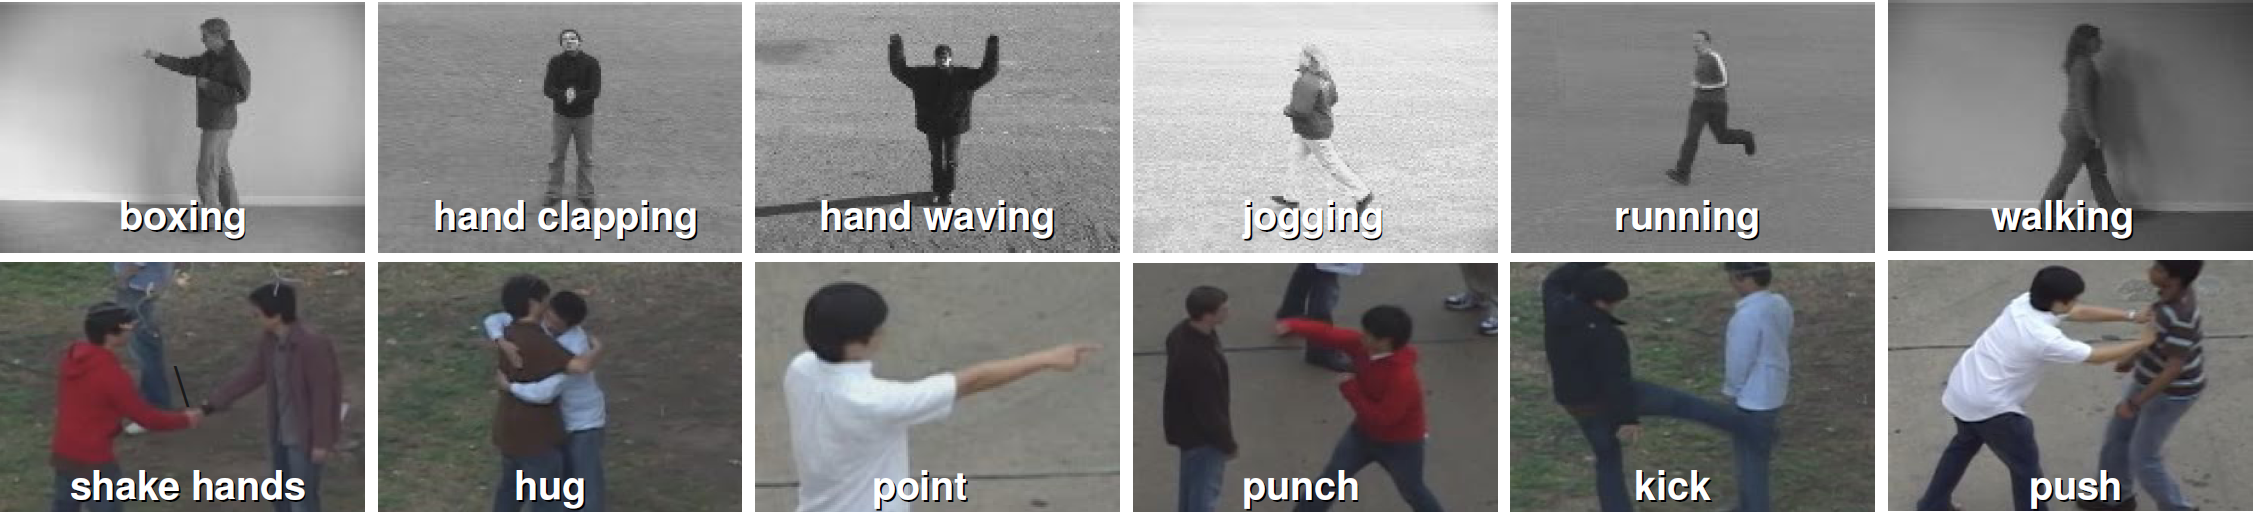
\includegraphics[width=1\linewidth]{fig/act/frames.png}
	\caption{Example frames of KTH (top row) and UT-interaction (bottom row) dataset}
	\label{fig/act/frames}
\end{figure}
%%%%%%%%%%%%%%%%%%%%%%%%%%%%%%%%%%%%%%%%%%%%%%%%%%%%%%%%%%%

% done 
The proposed system was evaluated on two public benchmarks, namely KTH dataset \cite{Schuldt2004} and UT-interaction dataset \cite{Ryoo2010}. 
Other existing approaches were compared with the proposed approach in terms of recognition accuracy. 
Run-time performance of the prototype system was also reported. A prototype action classification system was implemented in C++. Experiments were performed on an \emph{Intel Core}\texttrademark \; i7 $2.8$Ghz PC. It demonstrated real-time (about $15$ frames per second) and continuous action recognition performance. 
The prototype system was also deployed in a \emph{Intel Core 2 Duo} $2.4$Ghz labtop and ran at approximately $10$ frames per second on the KTH dataset. 
No multi-core optimisation was enabled in the prototype system. It is expected that the run-time performance can be further improved if the program code is optimised for multi-core processing units.

%The proposed method was tested on the well-known KTH dataset \cite{Schuldt2004} and the UT-interaction data \cite{Ryoo2010}, a more challenging set \cite{Ryoo2009}. Other published state-of-the-art approaches are compared with the proposed method in terms of recognition accuracy. Computational time of our method is also reported. The experimental prototype was implemented in C++ on a standard PC. The system runs in real-time and makes decisions in a continuous manner (see the supplementary video submitted). 


\subsection{KTH}

% done 
% dataset introduction KTH
The KTH dataset is an established benchmark for action recognition research. 
It contains sequences of six action classes captured in four different environments: boxing, hand-clapping, hand-waving, jogging, running and walking. 
The videos are taken with changing subjects, camera poses, scales and appearances, as illustrated in figure \ref{fig/act/frames}. 
The video sequences in KTH have a average length of $19$ second at $30$ frames per second. 
To recognise actions within a short response time, video snippet of $1$ second ($30$ frames) in length were extracted on-the-fly from the training and testing sequences. 
Each training subsequence (video snippet) was sampled in every $5$ frames, which was collected from the training dataset to build the classifiers. 
Testing subsequences were densely sampled from testing videos in a similar manner. 
Leave-one-out cross validation was used in the experiments. 

Most existing approaches were evaluated at the sequence level, where one class label was assigned to the entire testing video instead of individual frames or short subsequences. 
To put the proposed method in context, two different accuracy measures are defined: 
\begin{enumerate}
\item ``Snippet''(subsequence) level accuracy: It is directly measured at the subsequences level 
\item Sequence level accuracy: Class labels are determined by majority voting from the subsequences' classification labels 
\end{enumerate}

% done 
Table \ref{tab/act/exparam} summarises the parameters used in the experimental setup. They are set to obtain a balanced performance over accuracy, speed and generalisation. However, experimental results showed that small adjustments in the training parameters only brought marginal changes in overall accuracy. 
\begin{table}
\centering
\begin{tabular}{|c|c|c|}
\hline
\textbf{Parameter} & \textbf{Description} & \textbf{Value} \\
\hline
\multicolumn{3}{|c|}{\textbf{VFAST spatiotemporal interest points}}\\
\hline
$r_{XY}, r_{XT}, r_{YT}$ & radii of the Bresenham circles in VFAST & $3$ \\
$\delta^{FAST}_{XY}$ & thresholds of VFAST on the $XY$ plane& $35$\\
$\delta^{FAST}_{XT}$ & thresholds of VFAST on the $XT$ plane& $50$\\
$\delta^{FAST}_{YT}$ & thresholds of VFAST on the $YT$ plane& $50$\\
Dimensions$(\vpatch)$ & dimensions of video cuboid (x,y,t)& $(9,9,5)$ \\
\hline
\multicolumn{3}{|c|}{\textbf{Saptiotemporal semantic forest codebook}}\\
\hline
$stf_{dmax}$ & maximum depth of random forest codebook & $8$ \\
$stf_{bootstrap}$ & bootstrap factor of random forest codebook & $0.7$ \\
$stf_M$ & number of tree in random forest codebook & $15$ \\
\hline
\multicolumn{3}{|c|}{\textbf{Classification}} \\
\hline
$km_{dmax}$ & maximum depth of K-means forest & $3$ \\
$km_k$ & branching factor $k$ of K-means forest & $10$ \\
$rf_{dmax}$ & maximum depth of the BOST forest & $8$ \\
$rf_{bootstrap}$ & bootstrap factor of the BOST forest& $0.7$ \\
$rf_M$ & number of tree in the the BOST forest& $15$ \\ 
\hline
\end{tabular}
\caption{The training parameters used in the experiments. They are set to have balanced performance over accuracy, speed and generality.}
\label{tab/act/exparam}
\end{table}


% done 
Table \ref{tab/act/compare} presents a detailed comparison between our method and other state-of-the art approaches. The combined HSRM-BOST model demonstrated promising results, even only short video snippets are used to recognise actions. 
The confusion matrices in figure \ref{fig/act/confusion} shows that HSRM and BOST complemented each other to attain improved accuracy. 
Quantisation effects were soothed by the tree-based STF codebook and pyramid match kernel compared with the original spatiotemporal relationship match method in \cite{Ryoo2009}.

%%%%%%%%%%%%%%%%%%%%%%%%%%%%%%%%%%%%%%%%%%%%%%%%%%%%%%%%%%%
% Confusion matrices
%%%%%%%%%%%%%%%%%%%%%%%%%%%%%%%%%%%%%%%%%%%%%%%%%%%%%%%%%%%
\begin{figure}[ht]
\centering
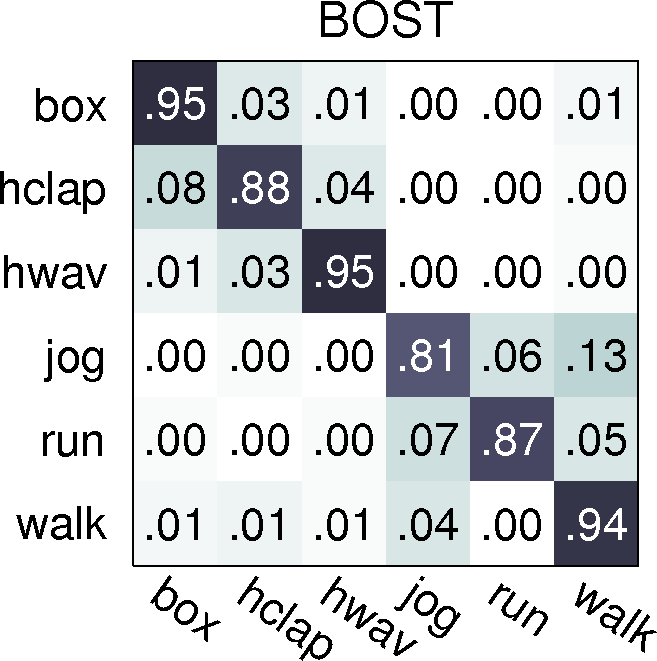
\includegraphics[width=0.32\linewidth]{fig/act/bost.png}
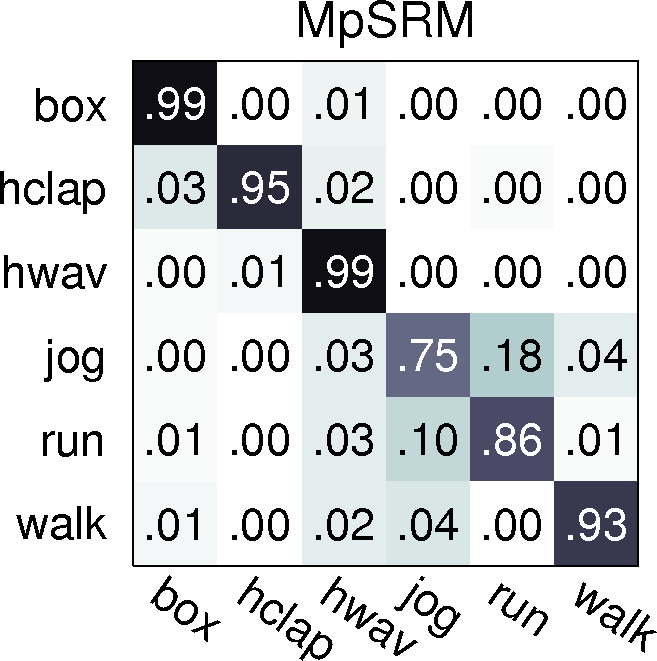
\includegraphics[width=0.32\linewidth]{fig/act/mpsrm.png}
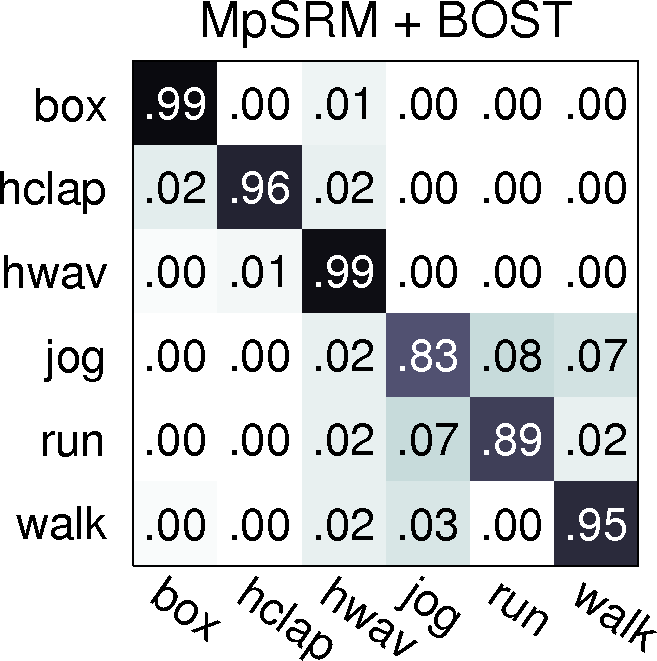
\includegraphics[width=0.32\linewidth]{fig/act/combine.png}
\caption{Confusion matrices of BOST (left), HSRM (middle), and combined classification(right) on KTH dataset}
\label{fig/act/confusion}
\end{figure}
%%%%%%%%%%%%%%%%%%%%%%%%%%%%%%%%%%%%%%%%%%%%%%%%%%%%%%%%%%%

%%%%%%%%%%%%%%%%%%%%%%%%%%%%%%%%%%%%%%%%%%%%%%%%%%%%%%%%%%%
% accuracy table: KTH
%%%%%%%%%%%%%%%%%%%%%%%%%%%%%%%%%%%%%%%%%%%%%%%%%%%%%%%%%%%
\begin{sidewaystable}
\centering
\begin{tabular}{|c|c|c|c|c|c|c|c|c|}
\hline
\textbf{Method} & \textbf{box} & \textbf{clap} & \textbf{wave} & \textbf{jog} & \textbf{run} & \textbf{walk} & \textbf{Overall} & \textbf{Protocol} \\
\hline
{HSRM + BOST} & \textbf{ \color{blue} 100.0} & \textbf{ \color{blue}96.0} & \textbf{ \color{blue}100} & \textbf{ \color{blue}86.0} & \textbf{ \color{blue}95.0} & \textbf{ \color{blue}97.0} & \textbf{ \color{blue}95.67} & sequence\\
{HSRM + BOST} & \textbf{ \color{blue} 99.0} & \textbf{ \color{blue} 96.6} & \textbf{ \color{blue}98.9} & \textbf{ \color{blue}82.6} & \textbf{ \color{blue}89.5} & \textbf{ \color{blue}94.8} & \textbf{ \color{blue} 93.55} & snippet\\
HSRM & 99.0 & 96.1 & 98.7 & 74.6 & 85.9 & 92.2 & \textbf{ 91.10} & snippet\\
SRM\cite{Ryoo2009} & 96.0 & 95.0 & 97.0 & 78.0 & 85.0 & 92.0 & \textbf{ 90.5} & sequence\\
\hline
Mined features \cite{Gilbert2009} & 100.0 & 94.0 & 99.0 & 91.0 & 89.0 & 94.0 & \textbf{\color{blue}{96.70}} & sequence\\
CCA \cite{Kim2007} & 98.0 & 100.0 & 97.0 & 90.0 & 88.0 & 99.0 & \textbf{ 95.33} & sequence\\
Neighbourhood** \cite{Kovashka2010} & - & - & - & - & - & - & \textbf{ 94.53} & sequence\\
Info. maximisation \cite{Liu2008} & 98.0 & 94.9 & 96.0 & 89.0 & 87.0 & 100.0 & \textbf{ 94.15} & sequence\\
Shape-motion tree \cite{Lin2009} & 96.0 & 99.0 & 96.0 & 91.0 & 85.0 & 93.0 & \textbf{ 93.43} & sequence\\
Vocabulary forest \cite{Mikolajczyk2008} & 97.0 & 96.0 & 98.0 & 88.0 & 93.0 & 87.0 & \textbf{ 93.17} & sequence\\
Point Clouds \cite{Bregonzio2009} & 95.0 & 93.0 & 99.0 & 85.0 & 89.0 & 98.0 & \textbf{ 93.17} & sequence\\
pLSA-ISA \cite{Wong2007} & 96.0 & 92.0 & 83.0 & 79.0 & 54.0 & 100.0 & \textbf{ 83.92} & sequence\\
\hline
\multicolumn{9}{p{0.9\linewidth}}{
\scriptsize * The length of subsequences called snippet is 30 frames. The depth of random forest classifier = $8$; For k-means forest classifier: K = $10$, depth = $3$. 
}\\
\multicolumn{9}{p{0.9\linewidth}}{
\scriptsize ** Classifiers were trained by a split dataset in separate scenarios. 
}\\
\end{tabular}
\caption{Accuracies on KTH data set by the proposed method and state-of-the-art methods. Leave one out cross validation (LOOCV) scheme was used.}
\label{tab/act/compare}
\end{sidewaystable}

%%%%%%%%%%%%%%%%%%%%%%%%%%%%%%%%%%%%%%%%%%%%%%%%%%%%%%%%%%%

% done 
Table \ref{tab/act/speed} shows the experimental results of run-time performance evaluation. Different from other sequence-level recognition approaches, a more realistic metric was designed to measure the algorithm efficiency. All stages in the recognition pipeline, including feature detection, feature extraction and classification, were timed. Average processing speed in frame per second is defined in equation \ref{eqn/act/fps}:
\begin{equation}
	\mbox{FPS} = \frac{\mbox{Total number of subsequences}\times\mbox{Average number of frames}}{\mbox{Total recognition time}} 
	\label{eqn/act/fps}
\end{equation} 
The proposed action recognition ran at $10$ to $20$ frames per second. 
The introduction of STF has greatly improved the performance in feature extraction and codeword generation without computing expensive features, outperforming k-means codebooks (see also Table \ref{tab/act/codebook}). Decision tree-based classifiers, namely random forest and kernel k-means forest, proved efficient solutions to match and recognise multi-dimensional codeword histograms over the traditional techniques, such as nearest neighbour and SVM. 

%%%%%%%%%%%%%%%%%%%%%%%%%%%%%%%%%%%%%%%%%%%%%%%%%%%%%%%%%%%
% Speed table
%%%%%%%%%%%%%%%%%%%%%%%%%%%%%%%%%%%%%%%%%%%%%%%%%%%%%%%%%%%
% DONE 
\begin{table}
\centering
\begin{tabular}{|c|c|c|}
	\hline 
	\backslashbox{\textbf{Process}}{\textbf{Dataset}} & \textbf{KTH} & \textbf{UT-interaction}\\
	\hline 
	VFAST detection & 66.1 & 35.1 \\ 
	STF \& BOST & 59.3 & 25.8 \\
	HSRM & 194.17 & 35.1 \\  
	Random forest & 1137.6 & 612.2 \\ 
	K-means forest & 67.1 & 428.1 \\
	\hline 
	\textbf{Total} & 18.98 & 10.02 \\
	\hline 
\end{tabular}
\caption{A list of the average recognition speed at different stages in frame per second (FPS)}
\label{tab/act/speed}
\end{table}

%%%%%%%%%%%%%%%%%%%%%%%%%%%%%%%%%%%%%%%%%%%%%%%%%%%%%%%%%%%
\subsection{UT-interaction Data set}
% dataset introduction UT
The UT-interaction dataset contains six classes of realistic human-to-human interactions, including shaking hands, pointing, hugging, pushing, kicking and punching, as visualised in figure \ref{fig/act/frames}. 
Challenging factors of this dataset include moving background, cluttered scene, camera jitters/zoom and clothing changes. 
In the experiments, the segmented UT-interaction dataset was used for evaluating the recognition accuracy and speed of the proposed action classification system. 
In table \ref{tab/act/utcompare}, the proposed method achieved better accuracy in recognising realistic human-human interactions than Ryoo \etal \cite{Ryoo2009}. 
With complex human interactions, using both local-appearance and structural cues in HSRM appeared more stable than BOST that uses only local-appearance. 
However, it still showed improvements in overall recognition accuracies in the combined approach. 
From table \ref{tab/act/speed}, the proposed system ran at real-time, with more than $10$ frames per second. 
The drop in run-time speed for the UT-interaction experiment is mainly due to the extra interest points detected from other moving objects in the backgrounds.

%%%%%%%%%%%%%%%%%%%%%%%%%%%%%%%%%%%%%%%%%%%%%%%%%%%%%%%%%%%
% accuracy table: UT-interaction
%%%%%%%%%%%%%%%%%%%%%%%%%%%%%%%%%%%%%%%%%%%%%%%%%%%%%%%%%%%
\begin{table}
	\centering
	\begin{tabular}{|c|c|c|c|c|}
		\hline 
		\backslashbox{\textbf{Action}}{\textbf{Method}} & \textbf{\color{blue}HSRM-BOST} & \textbf{HSRM} & \textbf{BOST} & \textbf{SRM}\cite{Ryoo2009} \\
		\hline 
		Shake & \textbf{\color{blue}100.0} & 90.0 & 80.0 & 75.0 \\ 
		Hug & \textbf{\color{blue}65.0} & 50.0 & 50.0 & 87.5 \\ 
		Point & \textbf{\color{blue}100.0} & 85.0 & 100.0 & 62.5 \\ 
		Punch & \textbf{\color{blue}85.0} & 65.0 & 65.0 & 50.0 \\ 
		Kick & \textbf{\color{blue}75.0} & 70.0 & 25.0 & 75.0 \\ 
		Push & \textbf{\color{blue}75.0} & 40.0 & 35.0 & 75.0 \\ 
		\hline 	
		\textbf{ Overall } & \textbf{\color{blue}83.33} & \textbf{66.67} & \textbf{59.16} & \textbf{70.8} \\ 
		\hline 
	\end{tabular}
	\caption{Sequence action recognition accuracy of the UT-interaction dataset. In the this experiment, leave one out cross validation (LOOCV) scheme were used.}
	\label{tab/act/utcompare}
\end{table}

\section{Discussion}
\label{sec/act/discussion}
%advantages: fast, fully utilises structural information
%limitation: still have some lookahead, not so powerful features, localisation not optimised
% This chapter has presented a novel solution for action recognition. Different from other published approaches, a major strength of our method is the run-time speed. Real-time performance is achieved by semantic texton forest which works on video pixels generating visual codewords in an extremely fast manner.  HSRM is proposed to capture both spatiotemporal structures and local-appearances of actions and ease quantisation effects based on STF. Furthermore, a novel fast interest point detector and application of random forest and kernel k-means forest classifiers contribute to the acceleration of recognition speed. Experimental results show the comparable accuracies of the proposed method compared to state-of-the-arts. A future challenge will be tackling more complex realistic human actions and partial occlusions, as well as requiring continuous action localisation with a real-time performance.
In this chapter, the topic of video-based action recognition is studied as an example of 3D object classification task. A novel real-time solution for video-based human action classification is proposed. 
Addressing the efficiency issues of existing techniques, a new real-time action recognition method is proposed. 
Real-time performance is achieved by semantic texton forests which work on video pixels generating visual codewords in an extremely fast manner. HSRM is also introduced to capture both spatiotemporal structures and local-appearances of video snippets. 
Furthermore, the application of random forests and kernel k-means forest classifiers contribute to the acceleration of recognition efficiency. 
The proposed system demonstrated comparable accuracies over state-of-the-art approaches in the experimental results. 
% Move to conclusions 
% Future challenges include tackling more complex realistic human actions and partial occlusions, as well as performing continuous action detection in real-time.
